\documentclass[12pt]{beamer}
\usetheme{Pittsburgh}
\usepackage[utf8]{inputenc}
\usepackage{amsmath}
\usepackage{amsfonts}
\usepackage{amssymb}
\usepackage{multirow}
\usepackage{graphicx}
\author{Russell Land}
\title{A Regression Analysis of Economic Performance}
\usepackage{ragged2e}
\setbeamercovered{transparent} 
\usecolortheme{dolphin}
\usepackage{adjustbox}
\usepackage{color}
\usepackage{pgfplots}
\usepackage{filecontents}
\pgfplotstableread[col sep = comma]{tgraph.csv}\mydata

\usepackage{verbatim}
\usepackage{tikz}
\usetikzlibrary{tikzmark}
\usepackage[style=FRAMEstyle]{mdframed}

\usepackage{tikz}
\usepackage{pgfplots}
\usetikzlibrary{shapes.geometric, arrows}

\tikzstyle{startstop} = [circle, minimum width=2.5cm, minimum height=1cm,text centered, draw=black]
\tikzstyle{io} = [circle, minimum width=2cm, minimum height=1cm, text centered, draw=black]
\tikzstyle{dot} = [circle, minimum width=0.5mm, minimum height=0.5mm, draw=white, fill = white]
\tikzstyle{arrow} = [thick, ->, >=stealth]
\tikzstyle{arrow2} = [thick, <->, >=stealth]


\institute{Georgia Southern University} 
\date{May 5, 2020} 
\subject{STAT 7134} 
\begin{document}

\begin{frame}
\titlepage
\end{frame}

\begin{frame}
\tableofcontents
\end{frame}

\section{Abstract}
\begin{frame}
\frametitle{Introduction}
This presentation will analyze data from an economic study, rating the performances of select firms using six different independent variables and one response variable. All of the variables used in this study are common financial measurements found daily in the Financial world.\\[3mm]
The data and some of the information in this presentation comes from a paper titled ``Using Linear Regression In The Analysis of Financial-Economic Performances." \cite{paper}
\end{frame}

\begin{frame}
\frametitle{Introduction}
The independent variables used in this study include:
\begin{itemize}
\item Good Money ($\text{GM}_i$)
\item Gross Operating Surplus ($\text{GOS}_i$)
\item Operating Gross Margin Rate ($R_{\text{mb}}$)
\item Cashflow/Turnover ($\text{CFR}_i$)
\item EBIT Margin ($\text{M}_{\text{EBIT}}$)
\item Total Debt Turnover ($\text{R}_{\text{Dt}}$)
\end{itemize}
and the response variable is:
\begin{itemize}
\item Economic Rate of Return ($\text{R}_{\text{ec}}$)
\end{itemize}
\end{frame}

\section{Data}
\begin{frame}
\frametitle{Data}
\begin{center}
\renewcommand{\arraystretch}{1.1}
{\tiny
\begin{tabular}{|r|c|c|c|c|c|c|c|}
\hline
\multirow{3}{*}{Firm} & Economic & Good  & Gross & Operating & Cash Flow/ & EBIT & Total\\
 & Rate of & Money & Operating & Gross & Turnover & Margin & Debt\\
 & Return & & Surplus & Margin Rate & & & Turnover\\
\hline
1  & 0.056 & 0.442 & 10383120 & 0.087 & 0.057 & 0.036 & 3.513 \\ \hline
2  & 0.076 & 0.022 & 9869544  & 0.070 & 0.027 & 0.042 & 2.565 \\ \hline
3  & 0.227 & 1.111 & 26685671 & 0.249 & 0.136 & 0.152 & 5.201 \\ \hline
4  & 0.041 & 0.003 & 12138277 & 0.110 & 0.024 & 0.076 & 1.400 \\ \hline
5  & 0.063 & 0.060 & 12032959 & 0.096 & 0.056 & 0.037 & 1.704 \\ \hline
6  & 0.077 & 0.004 & 10798008 & 0.083 & 0.012 & 0.080 & 0.905 \\ \hline
7  & 0.032 & 0.007 & 10696810 & 0.112 & 0.052 & 0.047 & 1.601 \\ \hline
8  & 0.281 & 2.452 & 23165418 & 0.212 & 0.194 & 0.165 & 9.502 \\ \hline
9  & 0.047 & 0.006 & 5421437  & 0.058 & 0.027 & 0.025 & 1.807 \\ \hline
10 & 0.174 & 0.043 & 13324530 & 0.132 & 0.063 & 0.117 & 1.937 \\ \hline
11 & 0.127 & 0.062 & 14044440 & 0.154 & 0.039 & 0.105 & 1.355 \\ \hline
12 & 0.110 & 0.006 & 13390931 & 0.149 & 0.058 & 0.096 & 1.344 \\ \hline
13 & 0.060 & 0.040 & 1492526  & 0.024 & 0.007 & 0.012 & 3.051 \\ \hline
14 & 0.245 & 0.025 & 20313159 & 0.227 & 0.046 & 0.179 & 1.358 \\ \hline
\end{tabular}}
\end{center}
\end{frame}


\begin{frame}
\frametitle{Data}
\begin{center}
\renewcommand{\arraystretch}{1.1}
{\tiny
\begin{tabular}{|r|c|c|c|c|c|c|c|}
\hline
\multirow{3}{*}{Firm} & Economic & Good  & Gross & Operating & Cash Flow/ & EBIT & Total\\
 & Rate of & Money & Operating & Gross & Turnover & Margin & Debt\\
 & Return & & Surplus & Margin Rate & & & Turnover\\
\hline
15 & 0.047 & 0.044 & 3735283  & 0.053 & 0.023 & 0.017 & 3.479 \\ \hline
16 & 0.122 & 0.087 & 13251207 & 0.153 & 0.083 & 0.094 & 3.600 \\ \hline
17 & 0.004 & 0.095 & 3989975  & 0.046 & 0.057 & 0.004 & 2.723 \\ \hline
18 & 0.135 & 0.177 & 14794181 & 0.222 & 0.034 & 0.136 & 0.703 \\ \hline
19 & 0.163 & 0.165 & 11972850 & 0.144 & 0.087 & 0.115 & 2.385 \\ \hline
20 & 0.060 & 0.044 & 3873616  & 0.082 & 0.023 & 0.030 & 1.400 \\ \hline
21 & 0.066 & 0.009 & 9019110  & 0.108 & 0.059 & 0.062 & 1.338 \\ \hline
22 & 0.116 & 0.164 & 3811847  & 0.056 & 0.003 & 0.043 & 1.878 \\ \hline
23 & 0.090 & 0.004 & 14018015 & 0.207 & 0.110 & 0.073 & 1.116 \\ \hline
24 & 0.150 & 0.074 & 11856849 & 0.159 & 0.061 & 0.099 & 1.243 \\ \hline
25 & 0.136 & 0.261 & 8376274  & 0.194 & 0.064 & 0.078 & 1.706 \\ \hline
26 & 0.137 & 0.025 & 15355836 & 0.279 & 0.092 & 0.132 & 0.795 \\ \hline
27 & 0.229 & 0.058 & 19331352 & 0.287 & 0.180 & 0.139 & 2.343 \\ \hline
28 & 0.120 & 0.346 & 4741264  & 0.073 & 0.039 & 0.046 & 3.295 \\ \hline
\end{tabular}}
\end{center}
\end{frame}

\section{Simple Linear Regression}
\subsection{Assumptions}
\begin{frame}
\frametitle{Regression Assumptions}
Before we finish building a model we need to establish the regression assumptions. These assumptions include:
\begin{enumerate}
\item The random error is distributed normally with mean 0 and variance $\sigma^2$.
\item Each observation is independent of one another.
\item The variance is constant for any value of $x$.
\end{enumerate}
\end{frame}

\subsection{Building Model}
\begin{frame}
\frametitle{Building Model}
For our simple linear regression analysis I am going to choose the variable $\text{M}_{\text{EBIT}}$ to be the regressor and the have the response variable be $\text{R}_{\text{ec}}$. Both of these measurement are dependent on the measurement EBIT. Here is a scatterplot of the two variables.
\begin{center}
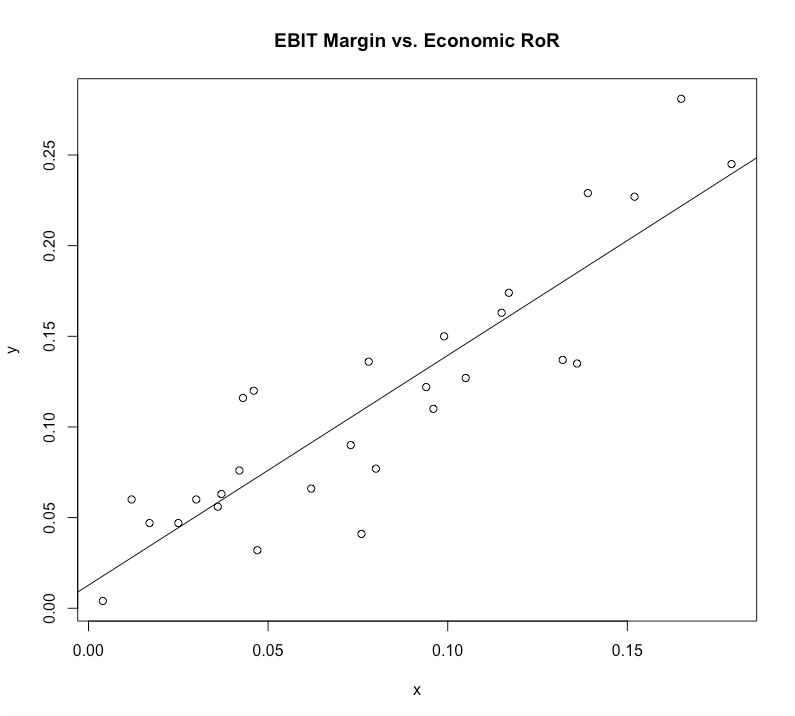
\includegraphics[scale=0.2]{SLRplot.png}
\end{center}
\end{frame}

\begin{frame}
\frametitle{Building Model}
From the scatterplot there seems to be evidence of an upward linear relationship between $X$ and $Y$. Next, let's estimate the regression coefficients for our model above. To estimate $\beta_0$ we can use $$\hat{\beta}_0=\bar{y}-\hat{\beta}_1\bar{x}$$ and we can estimate $\beta_1$ using $$\hat{\beta}_1=\frac{S_{xy}}{S_{xx}}$$ where
\begin{align*}
S_{xx}&=\sum_{i=1}^nx_i^2-\frac{1}{n}\left(\sum_{i=1}^nx_i\right)^2\\
S_{xy}&=\sum_{i=1}^nx_iy_i-\frac{1}{n}\left(\sum_{i=1}^nx_i\right)\left(\sum_{i=1}^ny_i\right)
\end{align*}
\end{frame}

\begin{frame}
\frametitle{Building Model}
After performing these calculations we obtain $\hat{\beta}_0=0.01271747$ and $\hat{\beta}_1=1.267282$. So, the estimated regression equation is: $$\hat{y}=0.013+1.267\hat{x}$$
\end{frame}

\subsection{Testing for Regression}
\begin{frame}
\frametitle{ANOVA Test}
Let's test for significance of regression. There are a few ways to do this; let's start by constructing an ANOVA table. Each observation can be treated as its own population. For an analysis of variance test we are testing the following hypothesis:
\begin{align*}
	&H_0:\;\mu_{y_1}=\mu_{y_2}=\cdots=\mu_{y_k}\\
	&H_1:\; \text{at least one $\mu_{y_i}$ is different}
\end{align*}
$$\iff$$
\begin{align*}
	&H_0:\; \sigma_B^2=\sigma_W^2=\sigma^2\\
	&H_1:\; \sigma_B^2>\sigma_W^2=\sigma^2
\end{align*}
\end{frame}

\begin{frame}
\frametitle{ANOVA Test}
\begin{center}
\resizebox{10cm}{5cm}{
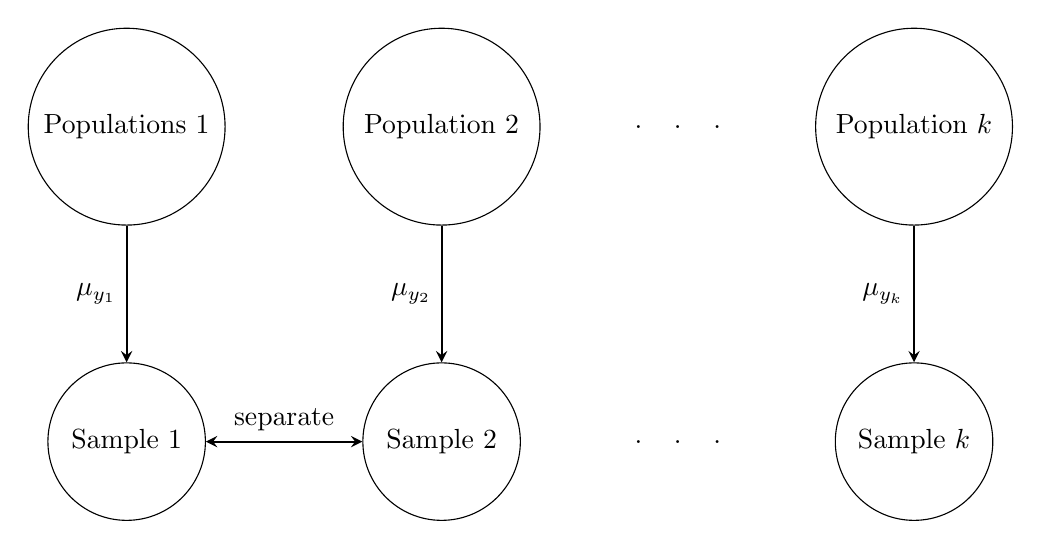
\begin{tikzpicture}[node distance = 4cm]
\node (start) [startstop] {Populations 1};
\node (next1) [startstop, right of=start] {Population 2};
\node (dot1) [dot, right of= next1, xshift = -1.5cm] {.};
\node (dot2) [dot, right of= dot1, xshift = -3.5cm] {.};
\node (dot3) [dot, right of= dot2, xshift = -3.5cm] {.};
\node (next2) [startstop, right of=dot3, xshift = -1.5cm] {Population $k$};
\node (in1) [io, below of=start] {Sample 1};
\node (in2) [io, below of=next1] {Sample 2};
\node (dot4) [dot, right of= in2, xshift = -1.5cm] {.};
\node (dot5) [dot, right of= dot4, xshift = -3.5cm] {.};
\node (dot6) [dot, right of= dot5, xshift = -3.5cm] {.};
\node (in3) [io, right of=dot6, xshift = -1.5cm] {Sample $k$};

\draw[arrow] (start) -- node[anchor = east] {$\mu_{y_1}$} (in1);
\draw[arrow] (next1) -- node[anchor = east] {$\mu_{y_2}$} (in2);
\draw[arrow] (next2) -- node[anchor = east] {$\mu_{y_k}$} (in3);
\draw[arrow2] (in1) -- node[anchor = south] {separate} (in2);
\end{tikzpicture}}
\end{center}
\end{frame}

\begin{frame}
\frametitle{ANOVA Test}
Now that we have established our hypothesis we can compute the ANOVA table in R. Below is the ANOVA table:
\begin{center}
{\scriptsize
\hspace*{-4mm}
\begin{tabular}{lccccc}
	\hline
	Source of Variation & Sum of Squares & Degrees of Freedom & Mean Square & $F_0$\\
	\hline
	Regression & 0.1039 & 1 & 0.1039 & 100.7644\\
	Residual & 0.0268 & 26 & 0.0010 &\\
	Total & 0.1307 & 27 & &\\
	\hline
\end{tabular}}
\end{center}

Our test statistic for the ANOVA test is 100.7644. To compute a p-value, we can use a built-in R function to obtain 1.958e-10. This number is very small and we have a significant test at very small levels of significance. At the 1\% level of significance we can conclude there is strong evidence for linear regression.
\end{frame}

\begin{frame}
\frametitle{Test for Regression}
There is another way to test for significance of linear regression under a simple linear regression model. We can calculate a confidence interval and check to see if 0 is contained in that interval. Let's find a 99\% confidence interval to test for significance of regression.
\end{frame}

\begin{frame}
\frametitle{Test for Regression}
The estimated parameter $\hat{\beta}_1$ is normally distributed with mean $\beta_1$ and variance $\sigma^2/S_{xx}$. Since the variance is unknown we can use the mean squared error to estimate it. The confidence interval for the estimated $\beta_1$ parameters is: $$\hat{\beta}_1-t_{\alpha/2,n-2}\cdot s_e\left(\hat{\beta}_1\right)\leq \beta_1\leq \hat{\beta}_1+t_{\alpha/2,n-2}\cdot s_e\left(\hat{\beta}_1\right)$$ Using R, our 99\% confidence interval for the regression parameter $\beta_1$ is: $$0.9164791\leq \beta_1\leq 1.6180857$$
\end{frame}

\begin{frame}
\frametitle{Test for Regression}
After using these two different methods, I think it is safe to assume there is significant evidence for linear regression. In other words, we are 99\% confident that the average slope of the regression model will be in the interval $$(0.9164791,1.6180857)$$ We could also perform a $t$-test to check for significance of regression, but this is already enough evidence.
\end{frame}

\begin{frame}
\frametitle{Making Predictions}
Let's try to predict the average Economic Rate of Return given that the EBIT Margin is 10\%. $$E[y|x=0.1]=0.013+1.267(0.1)=0.139$$ In fact, we can make many predictions. Let's make many predicts for the average Economic Rate of Return and future values of Economic Rate of Return.
\end{frame}

\begin{frame}
\frametitle{Making Predictions}
Below let's define the confidence intervals for both the average Economic Rate of Return and future values of Economic Rate of Return. For the average Economic Rate of Return: $$\hat{y}_0-t_{\alpha/2,n-2}\cdot s_e\left(\hat{y}_0\right)\leq \mu_{y|x_0}\leq \hat{y}_0+t_{\alpha/2,n-2}\cdot s_e\left(\hat{y}_0\right)$$ and the confidence interval for future values of Economic Rate of Return: $$\hat{y}_0-t_{\alpha/2,n-2}\cdot s_e\left(\Psi\right)\leq y_f\leq \hat{y}_0+t_{\alpha/2,n-2}\cdot s_e\left(\Psi\right)$$ The respective standard errors are: {\scriptsize $$s_e\left(\hat{y}_0\right)=\sqrt{\left(\frac{1}{n}+\frac{\left(x_0-\bar{x}\right)^2}{S_{xx}}\right)MS_{Res}}\qquad s_e\left(\Psi\right)=\sqrt{\left(1+\frac{1}{n}+\frac{\left(x_0-\bar{x}\right)^2}{S_{xx}}\right)MS_{Res}}$$}
\end{frame}

\begin{frame}
\frametitle{Making Predictions}
Now we can construct bounds for a 99\% confidence interval for both of these quantities. The graph is below:
\begin{center}
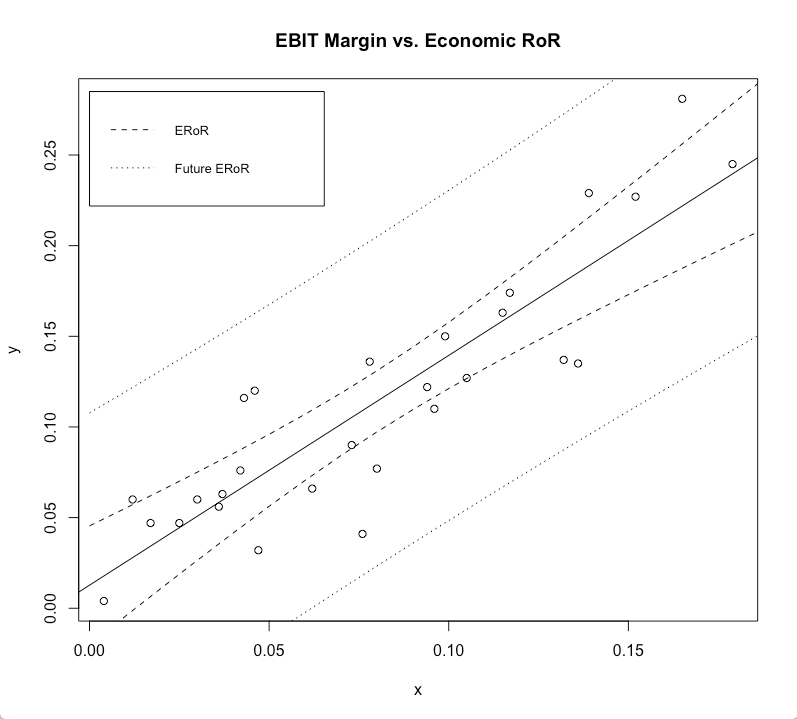
\includegraphics[scale=0.25]{99CI.png}
\end{center}
\end{frame}

\begin{frame}
\frametitle{R-Squared}
Beyond the confidence intervals, there are other ways to check for linearity. Another statistic is called the R-squared value. This measure is the ratio between the sum of squares regression and the total sum of squares. Another way to think of this measure is like: $$R^2=\frac{SS_R}{SS_T}=\frac{SS_T-SS_{Res}}{SS_T}$$ In other words, the more error there is in the model ($SS_{Res}$), the lower the R-squared value will be \cite{text2}. The R-squared value for this model is 0.795. This is a relatively high value, but there can be room for improvement. Since, this is predicting the economic performance of firms, this is acceptable.
\end{frame}

\section{Multiple Linear Regression}
\subsection{Building Model}
\begin{frame}
\frametitle{Building Model}
Now let's build a multiple linear regression model.\\[3mm]
For our multiple linear regression analysis, we will introduce five more regressors. The model will include all of the regressors from Table 1 with Economic Rate of Return as the response. We will use matrix formulation for the remainder of the regression analysis. The model is defined as: $$\vec{y}=X\vec{\beta}+\vec{\varepsilon}$$ where,
\end{frame}

\begin{frame}
\frametitle{Building Model}
$$\vec{y}=\begin{bmatrix}
	y_1\\
	y_2\\
	\vdots\\
	y_n\\
\end{bmatrix},\qquad X=\begin{bmatrix}
	1 & x_{11} & x_{12} & \cdots & x_{16}\\
	1 & x_{21} & x_{22} & \cdots & x_{26}\\
	\vdots & \vdots & \vdots & & \vdots\\
	1 & x_{n1} & \cdots & X_{n2} & \cdots x_{n6}\\
\end{bmatrix}$$ \vspace{1cm} $$\vec{\beta}=\begin{bmatrix}
	\beta_0\\
	\beta_1\\
	\vdots\\
	\beta_6\\
\end{bmatrix},\qquad \vec{\varepsilon}=\begin{bmatrix}
	\varepsilon_1\\
	\varepsilon_2\\
	\vdots\\
	\varepsilon_n\\
\end{bmatrix}$$
\end{frame}

\begin{frame}
\frametitle{Problems With Software}
When building the model there was an issue because the inverse matrix was turning singular in R. Now the matrix was not actually singular, but was computationally singular, meaning it involved precision that R cannot handle. To avoid this issue I will scale the data, then unscale after I build the model. Using the coefficients $\gamma_i$ and the scaled coefficients and $\beta$ as the unscaled coefficients, we can establish the relationship: $$\beta_0+\beta_1x_1+\cdots+\beta_px_p=\gamma_0+\gamma_1\left(\frac{x_1-\mu_1}{\sigma_1}\right)+\cdots+\gamma_p\left(\frac{x_p-\mu_p}{\sigma_p}\right)$$
\end{frame}

\begin{frame}
\frametitle{Building Model}
Using all of this, we are finally able to build our model: {\footnotesize $$y=-3.390-1.227x_1-4.845x_2-4.616x_3+2.256x_4+1.635x_5+1.364x_6$$}
\end{frame}

\subsection{Multicollinearity}
\begin{frame}
\frametitle{Multicollinearity}
I am speculating the reasons why this complication happened was because of highly correlated data. This issue was not a surprise as it was mentioned in the paper the data came from \cite{paper}. This concept is called multicollinearity. This is a problem that happens when the data is highly correlated and can be fixed by analyzing the the Variance Inflation Factors (VIF). Below are the VIFs for this model, calculated in R.
{\scriptsize
\begin{mdframed}
\verbatiminput{cor.txt}\verbatiminput{}
\end{mdframed}}
\end{frame}

\begin{frame}
\frametitle{Multicollinearity}
The rule of thumb for recognizing multicollinearity is VIF values above 10. Immediately we can see the regressors Operating Gross Margin Rate and Total Debt Turnover are potential risk for the model, so we will rid these of the model. Our new model now includes four regressors. Now let's rebuild our model without these: $$y=2.537+3.234x_1-5.002x_2+3.124x_4+1.505x_5$$
\end{frame}

\subsection{Test for Regression}
\begin{frame}
\frametitle{ANOVA Test}
Next, let's compute an ANOVA table to see if our model is significant. We can compute these all manually in R.
\begin{center}
{\scriptsize
\hspace*{-4mm}
\begin{tabular}{lccccc}
	\hline
	Source of Variation & Sum of Squares & Degrees of Freedom & Mean Square & $F_0$\\
	\hline
	Regression & 0.1148 & 4 & 0.0.0287 & 41.3876\\
	Residual & 0.0159 & 23 & 0.0007 &\\
	Total & 0.1307 & 27 & &\\
	\hline
\end{tabular}}
\end{center}
Our $F$ statistic is 41.3876, which corresponds to a p-value of 3.4488e-10. At the 1\% level of significance, we can conclude we have significant evidence of linear regression using the regressors listed above.
\end{frame}

\begin{frame}
\frametitle{Adjusted R-Squared}
The adjusted R-squared is a very helpful measure when more regressors are introduced to the model. The R-squared value increases as more regressors are introduced to the model, regardless of the importance of them. However, the adjusted R-squared addresses this issue by adjusting for this (dividing by degrees of freedom). The adjusted R-squared is defined as: $$R_{\text{adj}}^2=1-\frac{SS_{Res}/n-p}{SS_T/n-1}$$ In this model we have both a high adjusted R-squared value and a high R-squared value. These can be interpreted in the following way. We have an adjusted R-squared value of 0.8568, so around 86\% of the data is accounted for by the model.
\end{frame}

\begin{frame}
\frametitle{Test for Regression}
Now that we have established evidence of regression, let's test each coefficient using a $t$-test. Let's test whether the coefficient for Cash Flow contributes to the response. Let's test the following hypotheses:
\begin{align*}
	&H_0:\; \beta_4=0\\
	&H_a:\; \beta_4\neq 0
\end{align*}
The standard error can be calculated from the covariance matrix and the mean squared error. The standard error for the $i^{\text{th}}$ regression coefficient is defined as $\sqrt{C_{ii}\cdot MS_{Res}}$.
\end{frame}

\begin{frame}
\frametitle{Test for Regression}
The test statistic can be defined as: $$t=\frac{\hat{\beta}_4-\beta_4}{s_e\left(\hat{\beta}_4\right)}=\frac{3.124-0}{0.1791}=1.744$$ We can repeat this process for each coefficient. We can let software do the rest. We will test at the 5\% level of significance.
{\scriptsize
\begin{mdframed}
\verbatiminput{test.txt}\verbatiminput{}
\end{mdframed}}
\end{frame}

\begin{frame}
\frametitle{Test for Regression}
All coefficients are significant at the 5\% level except for $\beta_3$, the one we tested earlier. We can conclude that $\beta_0$, $\beta_1$, $\beta_2$, and $\beta_5$ contribute to the response variable at the 95\% confidence level.
\end{frame}

\subsection{Extra-Sum-of-Squares}
\begin{frame}
\frametitle{Extra-Sum-of-Squares Method}
Next, let's reduce our model one more time using the extra-sum-of-squares method. We will test the regressors $x_1$, $x_2$, and $x_5$. To do this method we will create two subsets for the regression coefficients, $\vec{\beta}_1=\left(\beta_0\;\beta_3\;\beta_4\;\beta_6\right)^t$ and $\vec{\beta}_2=\left(\beta_1\;\beta_2\;\beta_5\right)^t$. We want to test the following hypotheses:
\begin{align*}
	&H_0:\;\beta_1=\beta_2=\beta_5\\
	&H_a:\;\text{at least one $\beta_j\neq 0$}
\end{align*}
\end{frame}

\begin{frame}
\frametitle{Extra-Sum-of-Squares Method}
Now we can define the test statistic and compute it in R. $$F_0=\frac{MS_R\left(\vec{\beta}_2|\vec{\beta}_1\right)}{MS_{Res}}=0.0072/0.0006=11.0328$$ With the test statistic computed above, we can compute a p-value of 1.4716e-04. At the 1\% level of significance, we can conclude that the regressors $x_1$, $x_2$, and $x_5$ contribute to the response variable given that the other regressors are already in the model.
\end{frame}

\begin{frame}
\frametitle{Simultaneous Confidence Intervals}
Next, let's compute simultaneous confidence intervals using the Bonferoni Method at the 5\% confidence level using the optimal reduced model. For each $\beta_j$ the confidence interval can be defined as: $$\hat{\beta}_j-cv\cdot s_e\left(\hat{\beta}_j\right)\leq \beta_j\leq\hat{\beta}_j+cv\cdot s_e\left(\hat{\beta}_j\right)$$ where $cv$ is the critical value for the simultaneous confidence intervals.
\end{frame}

\begin{frame}
\frametitle{Simultaneous Confidence Intervals}
Finding this critical value is a little different than normal. Since it is a simultaneous critical value, we must consider all of the regressors at once. Consider the graph below.

\begin{center}
\resizebox{10cm}{4cm}{
\begin{tikzpicture}
	\begin{axis}[
		every non boxed x axis/.append style={x axis line style=-},
		no markers,
		axis x line=bottom,
		hide y axis=true,
		xtick={-1.2,0,1.2},
		ytick=\empty,
		xticklabels={$-t_{\alpha/2p,n-p}$,0,$t_{\alpha/2p,n-p}$},
		height=6cm,
		width=16cm,
		xmin = -4,
		xmax = 4,
		ymin = 0,
		ymax = 0.5
		]
	\addplot table[y index={1}]
		{\mydata}\closedcycle;
	\addplot+[mark=none,
		domain=-1.2:1.2,
		samples=200,
		fill=blue,
		fill opacity=0.2,
		draw=blue,
		area legend]{1/sqrt(2*pi)*exp(-x^2/2)} \closedcycle;  
	\put(190,45){$1-\frac{\alpha}{p}$};
	\put(100,30){$\frac{\alpha}{2p}$};
	\put(300,30){$\frac{\alpha}{2p}$};
	\end{axis}
\end{tikzpicture}}
\end{center}
The critical value can be computed in R as 2.700.
\end{frame}

\begin{frame}
\frametitle{Simultaneous Confidence Intervals}
Next, we can construct our confidence interval by finding the standard error for each coefficient. Below are the confidence interval.
{\scriptsize
\begin{mdframed}
\verbatiminput{SCI.txt}\verbatiminput{}
\end{mdframed}}

\vspace{2mm}

There are a few observations we can make from this simultaneous confidence interval. Two of the confidence intervals contain 0, indicating they are not significant. We have already establish however that our model is significant. One thing to be careful about is the fact that these values are already very close to 0, so these confidence intervals may not be very helpful.
\end{frame}

\section{Model Adequacy}
\subsection{Checking Model Adequacy}
\begin{frame}
\frametitle{Checking Model Adequacy}
The next topic is model adequacy. This idea will explore the initial assumptions we made at the beginning as whether they were correct assumptions or not. Statisticians may never know if their assumptions are correct, but there are many ways to sufficiently check. The main ways that we will check for our regression assumptions will be through:
\begin{enumerate}
\item Checking whether the current model is in-fact linear.
\item Checking if there is constant variance with respect to the random error.
\item Checking if the random error is normally distributed.
\end{enumerate}
\end{frame}

\begin{frame}
\frametitle{Checking Model Adequacy}
If these assumptions turn out to not be satisfied there may be a few actions taken. A transformation may be applied to change the model and perhaps fix the issue. We may also need to consider a different model, or in the worst case consider different sampling methods or re-sampling. We will only apply a transformation if necessary. Let's again state our model so we are clear what we are analyzing: $$y=\beta_0+\beta_1x_1+\beta_2x_2+\beta_5x_5+\varepsilon$$
\end{frame}

\begin{frame}
\frametitle{Checking Model Adequacy}
Our first method for checking model assumptions is to check for linearity. We have not calculated a complete regression analysis on the new model. We can do this in R.
{\scriptsize
\begin{mdframed}
\verbatiminput{newModel.txt}\verbatiminput{}
\end{mdframed}}
\end{frame}

\begin{frame}
\frametitle{Checking Model Adequacy}
There is an adjusted R-squared value of 0.8446 and an R-squared value of 0.8619. In my opinion, there is a clear linear relationship present. To further check this assumption, let's make plot of each regressor against the response variable.
\end{frame}

\begin{frame}
\frametitle{Checking Model Adequacy}
\begin{center}
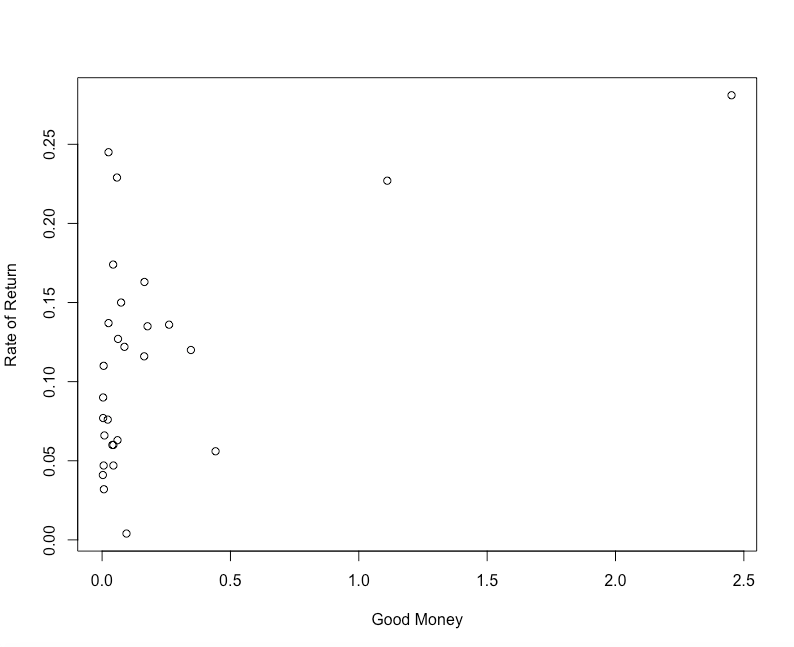
\includegraphics[scale=0.3]{pic1.png}
\end{center}
\end{frame}
\begin{frame}
\frametitle{Checking Model Adequacy}
\begin{center}
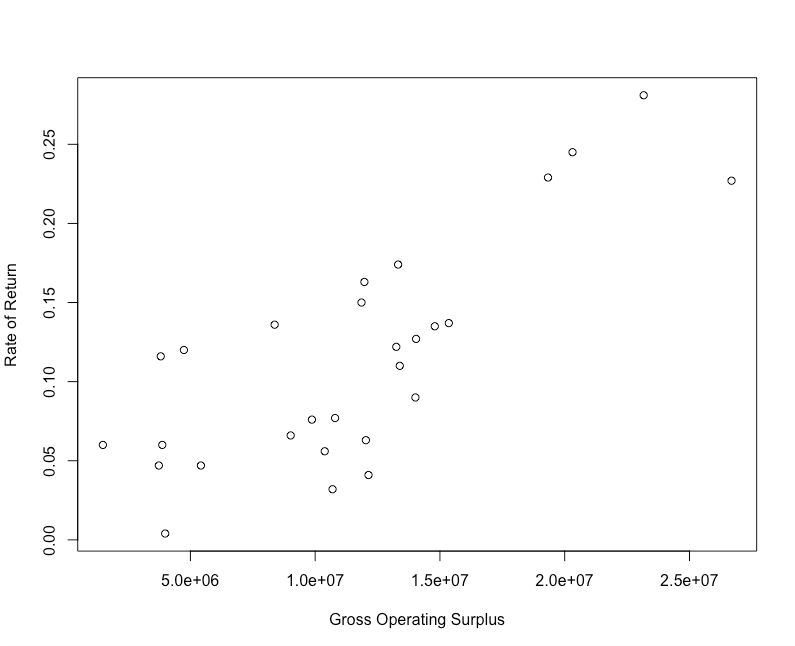
\includegraphics[scale=0.3]{pic2.png}
\end{center}
\end{frame}
\begin{frame}
\frametitle{Checking Model Adequacy}
\begin{center}
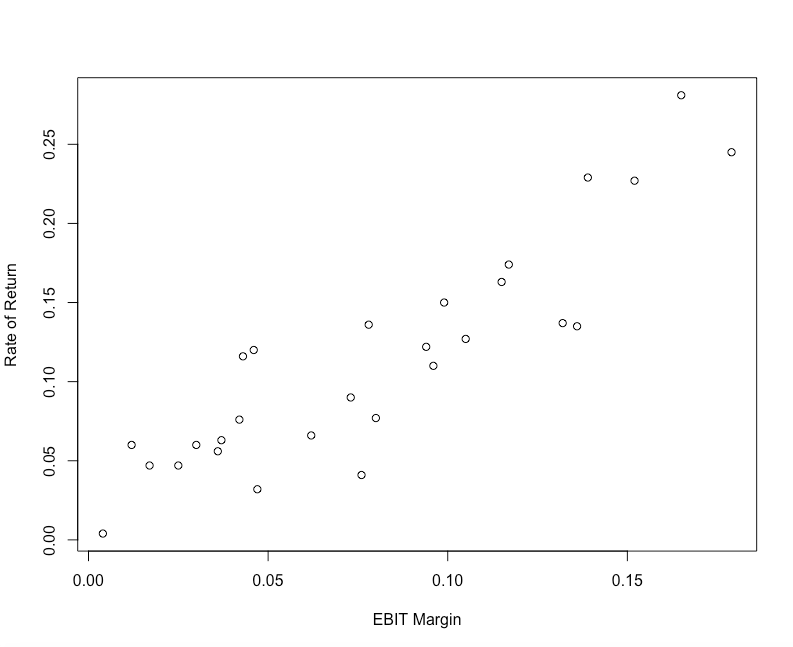
\includegraphics[scale=0.3]{pic3.png}
\end{center}
\end{frame}

\begin{frame}
\frametitle{Checking Model Adequacy}
There were very interesting results from these scatterplots. Even though our regression results from earlier pointed toward a strong linear relationship, we may need to reconsider our model. Let's move onto the assumption of constant variance. This can be checked by analyzing the residual plot against the fitted values. Also, also with the residuals plotted against the regressors as well. These plots will be below in that respective order.
\end{frame}

\begin{frame}
\begin{center}
\frametitle{Checking Model Adequacy}
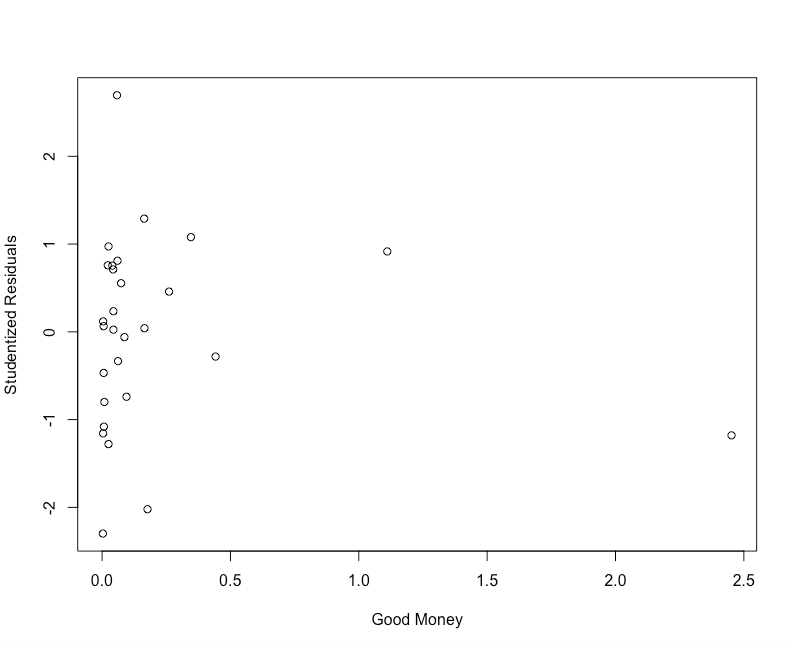
\includegraphics[scale=0.3]{pic4.png}
\end{center}
\end{frame}
\begin{frame}
\begin{center}
\frametitle{Checking Model Adequacy}
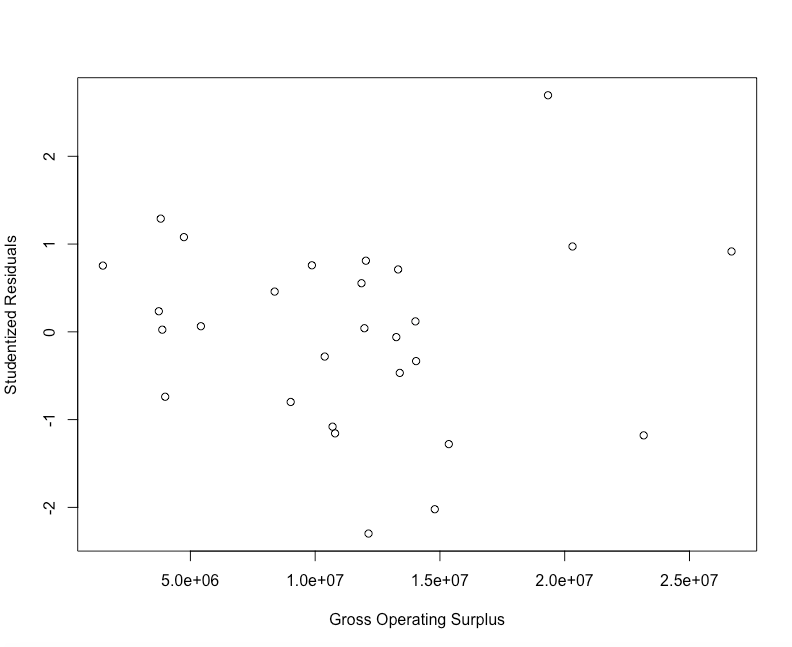
\includegraphics[scale=0.3]{pic5.png}
\end{center}
\end{frame}
\begin{frame}
\begin{center}
\frametitle{Checking Model Adequacy}
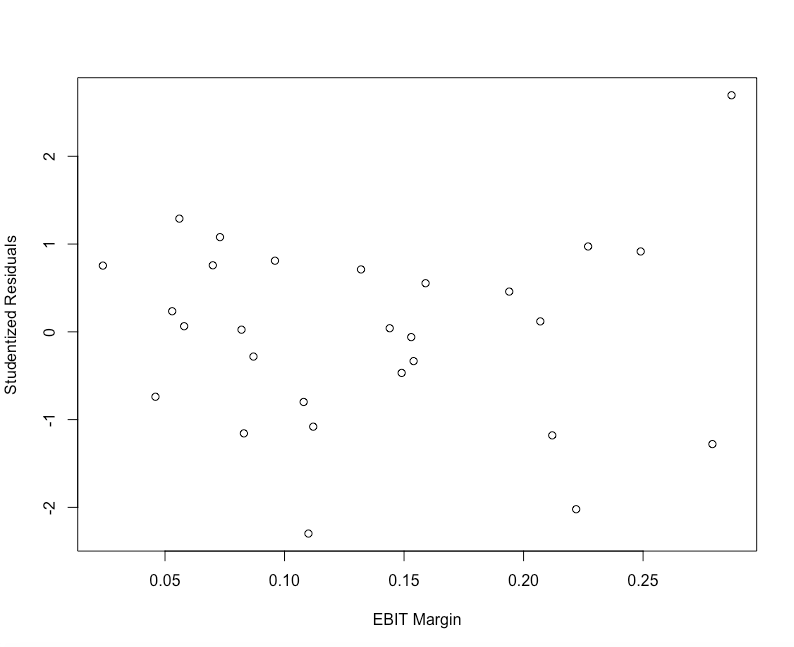
\includegraphics[scale=0.3]{pic6.png}
\end{center}
\end{frame}

\begin{frame}
\frametitle{Checking Model Adequacy}
From these residual plot and the scatterplot above it is beginning to become obvious of some assumption violations. The first residual plot is not ideal as there are a few outliers. The last residual plot is good enough, but again the second plot is not ideal either. Let's continue with the last regression assumption of normality before we make a decision on how to proceed. Below is a normal probability plot of the studentized residuals.
\end{frame}

\begin{frame}
\frametitle{Checking Model Adequacy}
\begin{center}
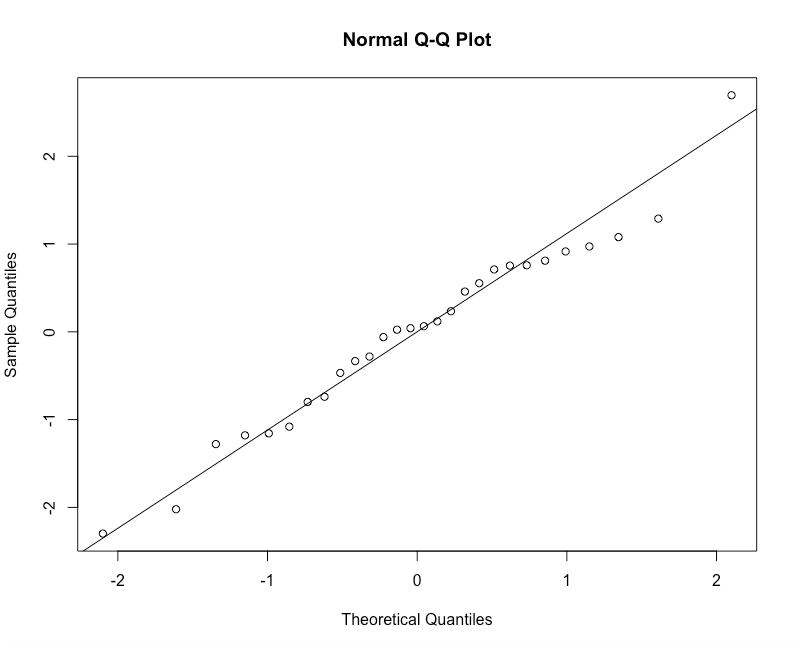
\includegraphics[scale=0.3]{pic7.png}
\end{center}
\end{frame}

\subsection{Transformation}
\begin{frame}
\frametitle{Transformation}
The assumption of normality is satisfied. Consider the other assumption violations for regression we will try a transformation to try to fix these assumptions. The main violation that I have found is the violation of linearity. If we can fix this, I believe our model can become adequate. After trying many different transformations\cite{text1}, consider the following model below: $$\sin^{-1}\left(\sqrt{y}\right)=\beta_0+\beta_1\log\left(x_1\right)+\beta_2x_2+\beta_5x_5+\epsilon$$ With these transformations defined let's rerun these assumptions tests and let's also run another regression analysis below.
\end{frame}

\begin{frame}
\frametitle{Transformation}
{\scriptsize
\begin{mdframed}
\verbatiminput{nmodel.txt}\verbatiminput{}
\end{mdframed}}
\end{frame}

\begin{frame}
\frametitle{Transformation}
{\tiny
\begin{mdframed}
\verbatiminput{resid.txt}\verbatiminput{}
\end{mdframed}}
\end{frame}

\begin{frame}
\frametitle{Transformation}
\begin{center}
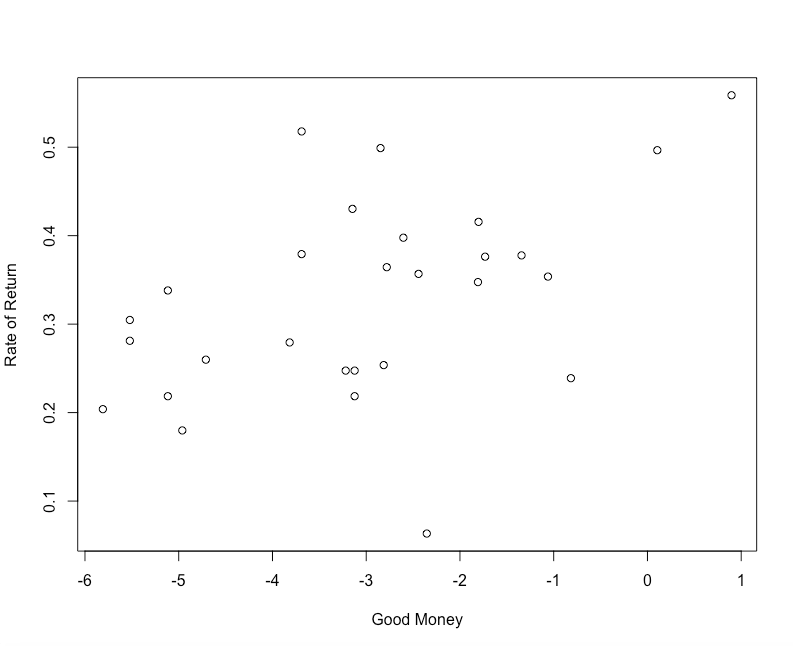
\includegraphics[scale=0.3]{pic11.png}
\end{center}
\end{frame}
\begin{frame}
\frametitle{Transformation}
\begin{center}
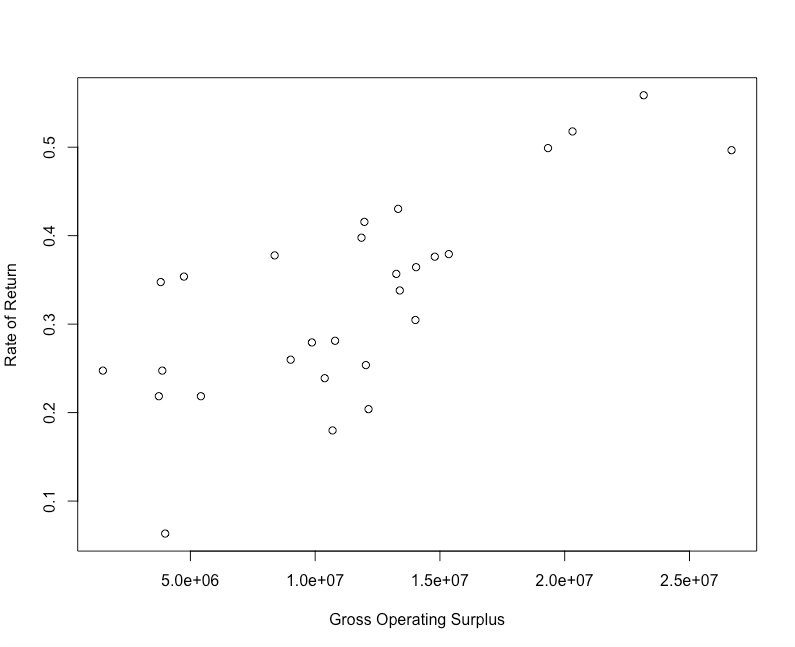
\includegraphics[scale=0.3]{pic12.png}
\end{center}
\end{frame}
\begin{frame}
\frametitle{Transformation}
\begin{center}
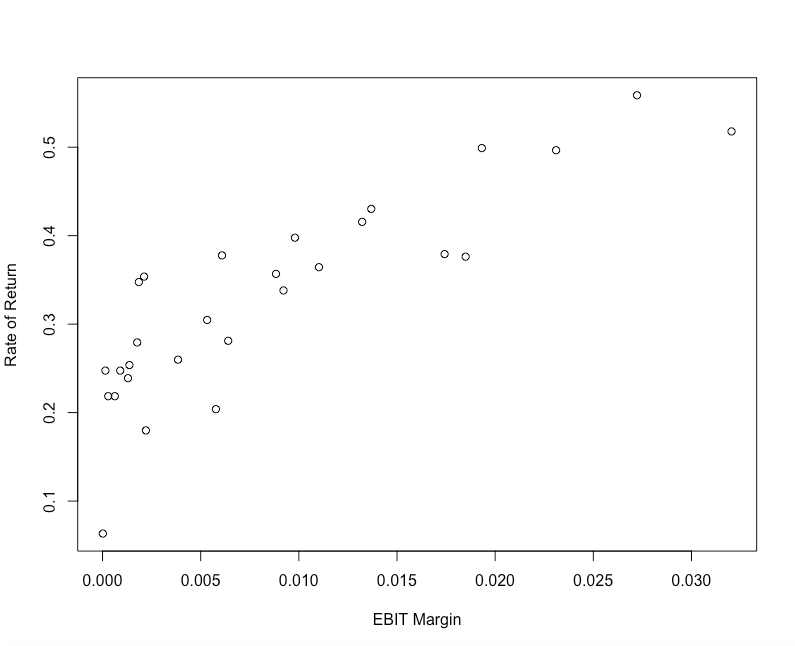
\includegraphics[scale=0.3]{pic13.png}
\end{center}
\end{frame}

\begin{frame}
\frametitle{Transformation}
\begin{center}
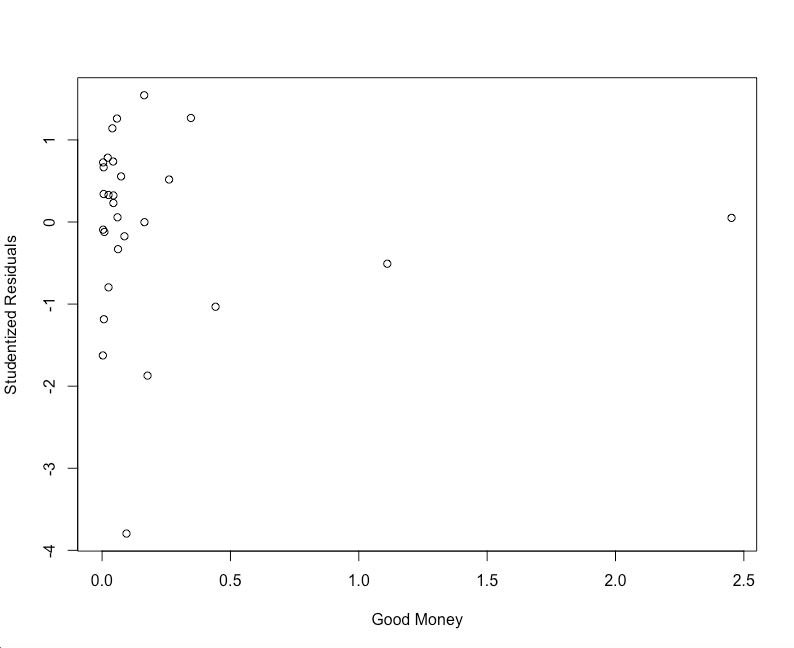
\includegraphics[scale=0.3]{pic14.png}
\end{center}
\end{frame}
\begin{frame}
\frametitle{Transformation}
\begin{center}
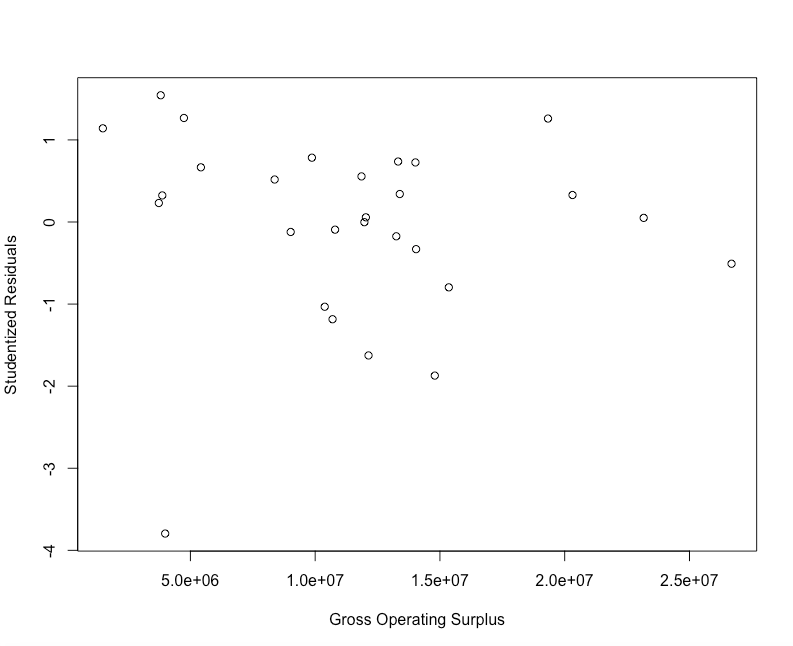
\includegraphics[scale=0.3]{pic15.png}
\end{center}
\end{frame}
\begin{frame}
\frametitle{Transformation}
\begin{center}
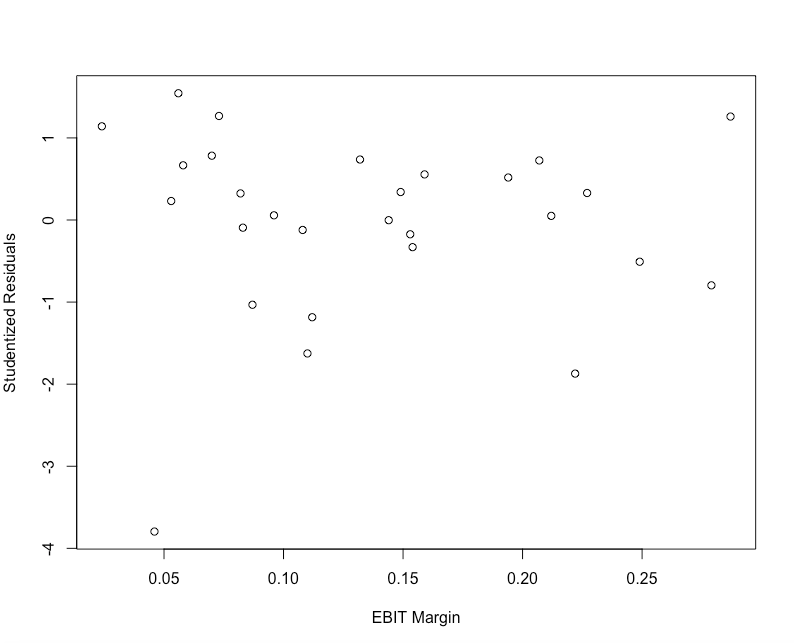
\includegraphics[scale=0.3]{pic16.png}
\end{center}
\end{frame}

\begin{frame}
\frametitle{Transformation}
\begin{center}
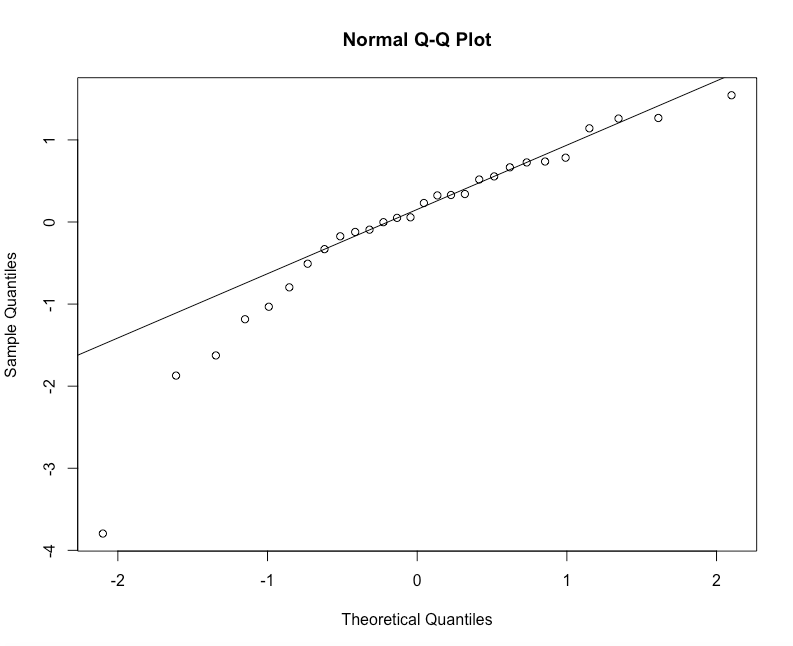
\includegraphics[scale=0.3]{pic17.png}
\end{center}
\end{frame}

\begin{frame}
\frametitle{Transformation}
The transformation looks like it helped our assumption of linearity. The scatterplots seemed to have improved some. However, the other assumptions mentioned earlier do not seem to have improved. To conclude, I think we should stick with the transformed model. The studentized residuals only produce one outlier, while the rest are below 2. This is good sign.
\end{frame}

\section{Conclusion}
\begin{frame}
\frametitle{Conclusion}
The regression analysis above revealed some interesting results, and unexpected results at that. I did not expect the issue arising regarding the computational singularity with R. This was an issue that was finally fixed with a lot of different attempts. Regardless, I believe that our initial simple linear regression analysis with the one regressor EBIT Margin was a superior model to the optimal model found in the multiple linear regression analysis. All of the other regression just seemed to add `noise' to the data. Sometimes a best model is not always the more complicated model. This project just goes to show that making economic prediction can be very difficult and unreliable at times.
\end{frame}

\begin{frame}
\frametitle{References}
\bibliographystyle{plain}
\bibliography{bibliography}
\end{frame}

\end{document}